\documentclass[useAMS,usenatbib]{mnras}
\usepackage{color}
\usepackage{graphicx}
\usepackage{dcolumn}
\usepackage{bm}
\usepackage{amssymb}
\usepackage{latexsym}
\usepackage[T1]{fontenc}
\usepackage{aecompl} 

\newcommand{\hMsun}{{\ifmmode{h^{-1}{\rm
        {M_{\odot}}}}\else{$h^{-1}{\rm{M_{\odot}}}$~}\fi}} 
\newcommand{\hMpc}{{\ifmmode{h^{-1}{\rm Mpc}}\else{$h^{-1}$Mpc }\fi}}

%%%%%%%%%%%%%%%%%%%%%%%%%%%%%%%%%%%%%%%%%%%%%%%%

\begin{document}

\title[Constraining CPL via clustering shells of BOSS]{Cosmological constraints via clustering shells: 
constraining the Chevallier-Polarski-Linder parametrization using the SDSS-III BOSS data}

\author[Xiao-Dong~Li, Yuting Wang, Gong-bo Zhao, Changbom Park, Hyunbae Park, Cristiano G. Sabiu]
{ Xiao-Dong Li$^{1,2,\dagger}$,  Yuting Wang$^{2}$, Gong-bo Zhao$^{2}$, Changbom Park$^{1}$, Hyunbae Park$^{2}$, Arman Shafieloo$^{2}$,
Cristiano G. Sabiu$^{2,\star}$, Juhan Kim$^{3,1}$\\
$^1$School of Physics, Korea Institute for Advanced Study, 85 Heogi-ro, Dongdaemun-gu, Seoul 130-722, Korea\\
$^2$Korea Astronomy and Space Science Institute, 776, Daedeokdae-ro, Yuseong-gu, Daejeon, 305-348, Korea\\
$^3$Center for Advanced Computation, Korea Institute for Advanced Study, 85 Hoegi-ro, Dongdaemun-gu, Seoul 130-722, Korea\\
$^{\dagger}$xiaodongli@kias.re.kr\\
$\star$Corresponding Author: csabiu@kasi.re.kr}




%\date{Accepted 1988 December 15. Received 1988 December 14; in original form 1988 October 11}

% \begin{keywords}
% methods: data analysis -- methods: statistical -- Galaxies:
% kinematics and dynamics -- Cosmology: observations -- large-scale
% structure of universe
% \end{keywords}

\pagerange{\pageref{firstpage}--\pageref{lastpage}} \pubyear{2002}

\maketitle

\label{firstpage}

\begin{abstract}
Li et al. 2016 proposed to use the redshift dependence of the Alcock-Paczynski to constrain cosmological parameters.
Tight constraints on $\Omega_m$ and $w$ were derived using the SDSS-III BOSS galaxies.
In this paper we extend the analysis to put constraints on the Chevallier-Polarski-Linder parametrization.
To explore the high dimension parameter space, we measure the 2-point correlation function in some fiducial cosmology,
and map out its value in the other cosmologies.
%The accuracy is below 1\%.
We derive constraints of ...
\end{abstract}

% \begin{keywords}
% circumstellar matter -- infrared: stars.
% \end{keywords}

\section{Introduction}


DE is very important. 
\citep{Li2016} proposed to use redshift dependence of AP to constrain cosmological parameters.
Very good results obtained from SDSS-III BOSS galaxies.

\citep{Li2016} only considered constraints on $\Omega_m$ and $w$ in a flat Universe.
In this paper we extend to CPL parameters.




\section{Methodology}


The 2pCF of the 1\,133\,326 BOSS DR12 galaxies are measured in six redshift bins of
$0.150<z_1<0.274<z_2<0.351<z_3<0.430<z_4<0.511<z_5<0.572<z_6<0.693$.
To capture the information of small-scale anisotropic clustering we compute the quantity
$\xi_{\Delta s} (\mu) \equiv \int_{s_{\rm min}}^{s_{\rm max}} \xi (s,\mu)\ ds$
with $s_{\rm min}=6 h^{-1} {\rm Mpc},\ s_{\rm max}=40 h^{-1} {\rm Mpc}$.
We further normalise it as 
$\hat\xi_{\Delta s}(\mu) \equiv \frac{\xi_{\Delta s}(\mu)}{\int_{0}^{\mu_{\rm max}}\xi_{\Delta s}(\mu)\ d\mu}$
to abondon the amplitude information which has nothing to do with the Alcock-Paczynski test and is sensitive to the galaxy bias.
The ``correct'' cosmologies are selected by assessing the amount of redshift evolution of $\hat\xi_{\Delta s}$,
via a $\chi^2$ function of 
\begin{equation}
 \chi^2\equiv \sum_{i=2}^{6} \sum_{j_1=1}^{n_{\mu}} \sum_{j_2=1}^{n_{\mu}} {\bf p}(z_i,\mu_{j_1}) ({\bf Cov}_{i}^{-1})_{j_1,j_2}  {\bf p}(z_i,\mu_{j_2})
\end{equation}
where ${\bf p}(z_i,\mu_{j})$ is the redshift evolution of clustering with respective to the lowest redshift bin,
with systematic effects subtracted:
$ {\bf p}(z_i,\mu_{j}) \equiv\  \left[\hat\xi_{\Delta s}(z_i,\mu_j)-\hat\xi_{\Delta s}(z_1,\mu_j)\right] - \left[\hat\xi_{\Delta s}(z_i,\mu_j)-\hat\xi_{\Delta s}(z_1,\mu_j)\right]_{\rm sys}$.
We use a number of $n_{\mu}$=20, 21, ... 25 bins for the value of $\hat\xi_{\Delta s}(\mu)$.
For the removal of fiber collision and the strong FoG near the LOS cut we take a cut $\mu_{\rm max} = 0.97$.

The systematics are estimated on mock catalogues from Horizon Run 4 (HR4) \cite{HR4},
an N-body simulation with box size $L={3150}$ $h^{-1}$Mpc, number of particles $6300^3$,   
initial redshift $z_{i}=100$, and WMAP5 cosmological parameter 
$(\Omega_{b},\Omega_{m},\Omega_\Lambda,h,\sigma_8,n_s)$  = (0.044, 0.26, 0.74, 0.72, 0.79, 0.96) \citep[]{komatsu 2011}.
Mock galaxy samples are produced using a modified version of the one-to-one correspondence scheme \citep{hong2016}. 
The covariance matrice ${\bf Cov}$ are computed from the 2,000 sets of MultiDark PATCHY mock catalogues \citep{MDPATCHY}.
The statistical bias and scattering in the likelihood function (due to the finite number of mocks in covariance estimation) 
are corrected following Hartlap et al. (2006) and Percival et al. (2014).

In \cite{Li2016} the likelihood contour of $\Omega_m-w$ was constructed by
measuring the 2PCF 3,375 times,
using 3D positions of BOSS galaxies under 71$\times$45 sets of cosmological parameters
($0.06\leq \Omega_m\leq 0.41$, $-1.5 \leq w \leq -0.4$).
It took 1 months using 500 cores of the KIAS baekdu cluster.
It would be too expensive to redo the above computation on a 3D grid of $\Omega_m-w_0-w_a$,
%and explore the parameter space of dynamical dark energy.
so here we take an approach  of ``approxmiate 2PCF'', described as follows.

The number counts DD, DR, RR as are measured in a fiducial cosmology
-- which are taken as the $\Omega_m=0.26$ $\Lambda$CDM --
and ``translated'' to the measurements in a ``target'' cosmologies using 
\begin{eqnarray}
 s_{\rm target} = s_{\rm fiducial} \sqrt{\alpha_{\parallel}^2 \mu_{\rm fiducial}+\alpha_{\bot}(1-\mu_{\rm fiducial}^2)}, \\
 \mu_{\rm target} = \mu_{\rm fiducial} \frac{\alpha_\parallel}
 {\sqrt{\alpha_{\parallel}^2 \mu_{\rm fiducial} +\alpha_{\bot}(1-\mu_{\rm fiducial}^2)}}
\end{eqnarray}
where $\alpha_{\bot}\equiv D_{A,\rm target}/D_{A,\rm fiducial}$,
$\alpha_{\parallel}\equiv H_{\rm fiducial}/H_{\rm target}$.
and values of $D_A$ and $H$ are computed in the effective redshifts of the six bins.
In the fiducial cosmology
we measure $\xi(s,\mu)$ in an ultra high resolution of
$\Delta s = 0.2 {\rm Mpc/h}$, $\Delta \mu = 1/600$,
%Let us call this ``approximate 2pCF'' method.
%to obtain the accurate number counts 
so that the small $(s,\mu)$ ``pixels'' can be grouped to infer 
the number counts in other cosmologies with large pixels of 
$\Delta s = 1 {\rm Mpc/h}$, $\Delta \mu = 1/120$.
%in the fiducial cosmology and group the bins in the target cosmology.
The ``edge effects'' (one small pixel belongs to more than one large pixel) 
are carefully treated to reduce the error.
We found that using the approximated method the computed 
$\hat\xi_{\Delta s}(\mu)$ in non-ficucial cosmologies suffer from
an error of $\approx0.5\%$, which is 10 times smaller than 
the statistical noise.

%We have checked that our result is insensitive to the choices of $n_\mu$ and $\mu_{\rm max}$,
%the systematics correction, the number of mocks for covariance matrix estimation.




\section{Results}


Combining our method with CMB+BAO+JLA+$H_0$ we derive the following constraints on CPL parameters
\begin{equation}
%\Omega_m = 0.300 \pm 0.008, w_0 = -1.056 \pm 0.061, w_a = -0.04 \pm 0.27,
    %1  0.2999656E+00  0.7616334E-02  0.2958745E+00  0.3035033E+00  0.2878169E+00  0.3132870E+00   \Omega_m
    %2  0.6904801E+00  0.8675444E-02  0.6808558E+00  0.6993898E+00  0.6722945E+00  0.7052207E+00   h
    %3 -0.1056468E+01  0.6096323E-01 -0.1116874E+01 -0.9965903E+00 -0.1175041E+01 -0.9287388E+00   w
    %4 -0.3808376E-01  0.2716607E+00 -0.3105235E+00  0.2321461E+00 -0.6033103E+00  0.4782076E+00   w_a    
\Omega_m = 0.301 \pm 0.008, w_0 = -1.042 \pm 0.067, w_a = -0.07 \pm 0.29,    
%    1  0.3014353E+00  0.7759923E-02  0.2974325E+00  0.3048882E+00  0.2889838E+00  0.3152269E+00   \Omega_m
%    2  0.6887652E+00  0.8760036E-02  0.6797134E+00  0.6978279E+00  0.6703971E+00  0.7044224E+00   h
%    3 -0.1041626E+01  0.6732817E-01 -0.1107730E+01 -0.9768319E+00 -0.1172149E+01 -0.8979017E+00   w
%    4 -0.7173374E-01  0.2860547E+00 -0.3572176E+00  0.2107347E+00 -0.6775045E+00  0.4558817E+00   w_a    
\end{equation}
while the results without adding our method are
\begin{equation}
\Omega_m = 0.309 \pm 0.010, w_0 = -0.938 \pm 0.109, w_a = -0.38 \pm 0.41.
%    1  0.3086006E+00  0.9639142E-02  0.3039045E+00  0.3131096E+00  0.2926126E+00  0.3249674E+00   \Omega_m
%    2  0.6809952E+00  0.1054577E-01  0.6703974E+00  0.6916269E+00  0.6605231E+00  0.7026640E+00   h
%    3 -0.9377990E+00  0.1092489E+00 -0.1046659E+01 -0.8303874E+00 -0.1149980E+01 -0.7142246E+00   w
%    4 -0.3777249E+00  0.4069512E+00 -0.7694896E+00  0.1941066E-01 -0.1285417E+01  0.3473089E+00   w_a
\end{equation}


The result is fully consistent with a dark energy component having no evolution.
Adding the AP likelihood reduced the statistical errors by $\sim$30-40\%,
reduced the 95.4\% CL $w_0-w_a$ contour by 47\%.
This reveals the power of the our method in constraining the redshift evolution of dark energy.

\begin{figure*}
   \centering{
   %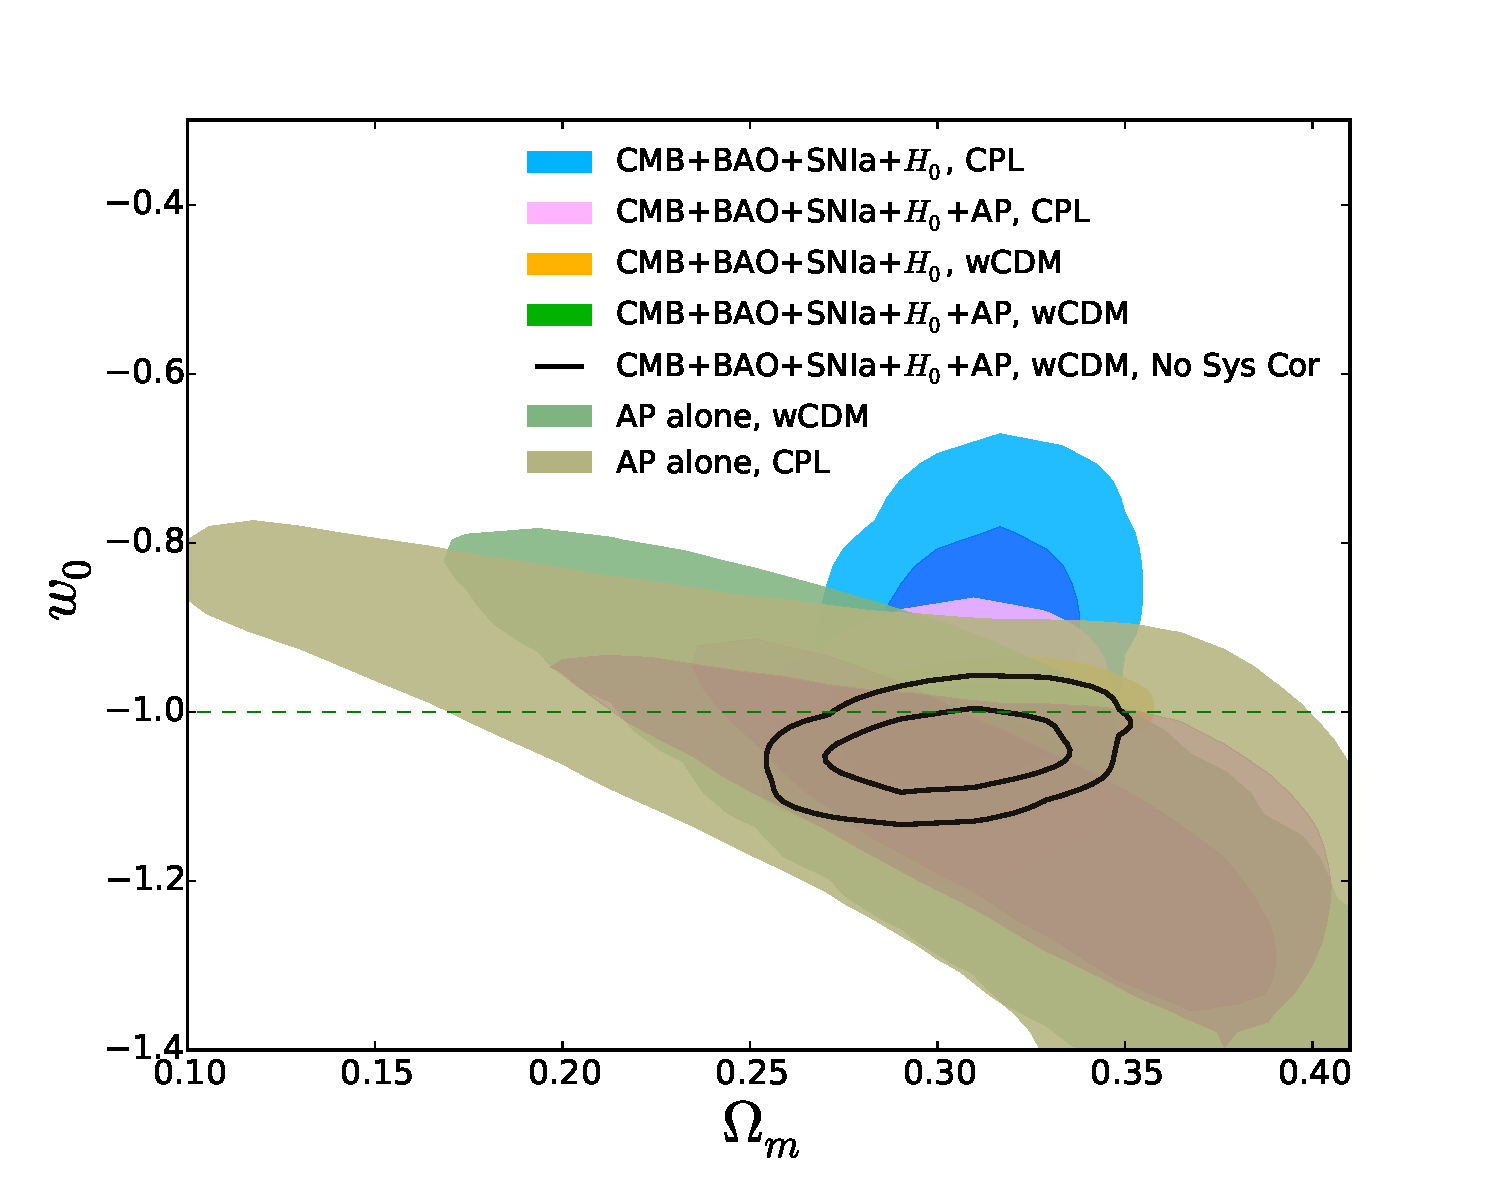
\includegraphics[width=9cm,natwidth=4,natheight=4]{figCPL_a.pdf}
   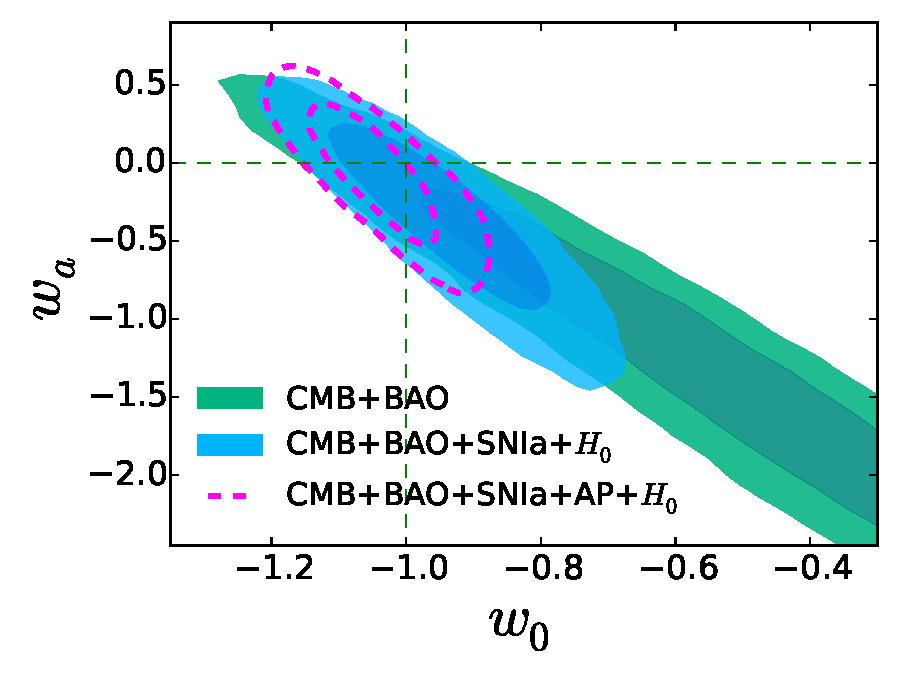
\includegraphics[width=7cm,natwidth=4,natheight=4]{figCPL_b.pdf}
   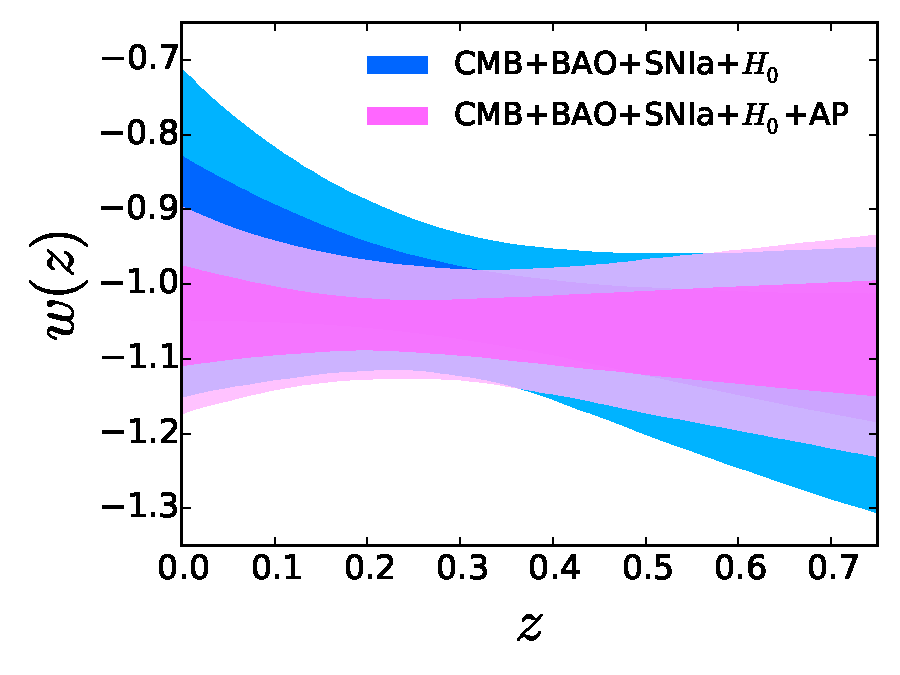
\includegraphics[width=7cm,natwidth=4,natheight=4]{figCPL_d.pdf}
   %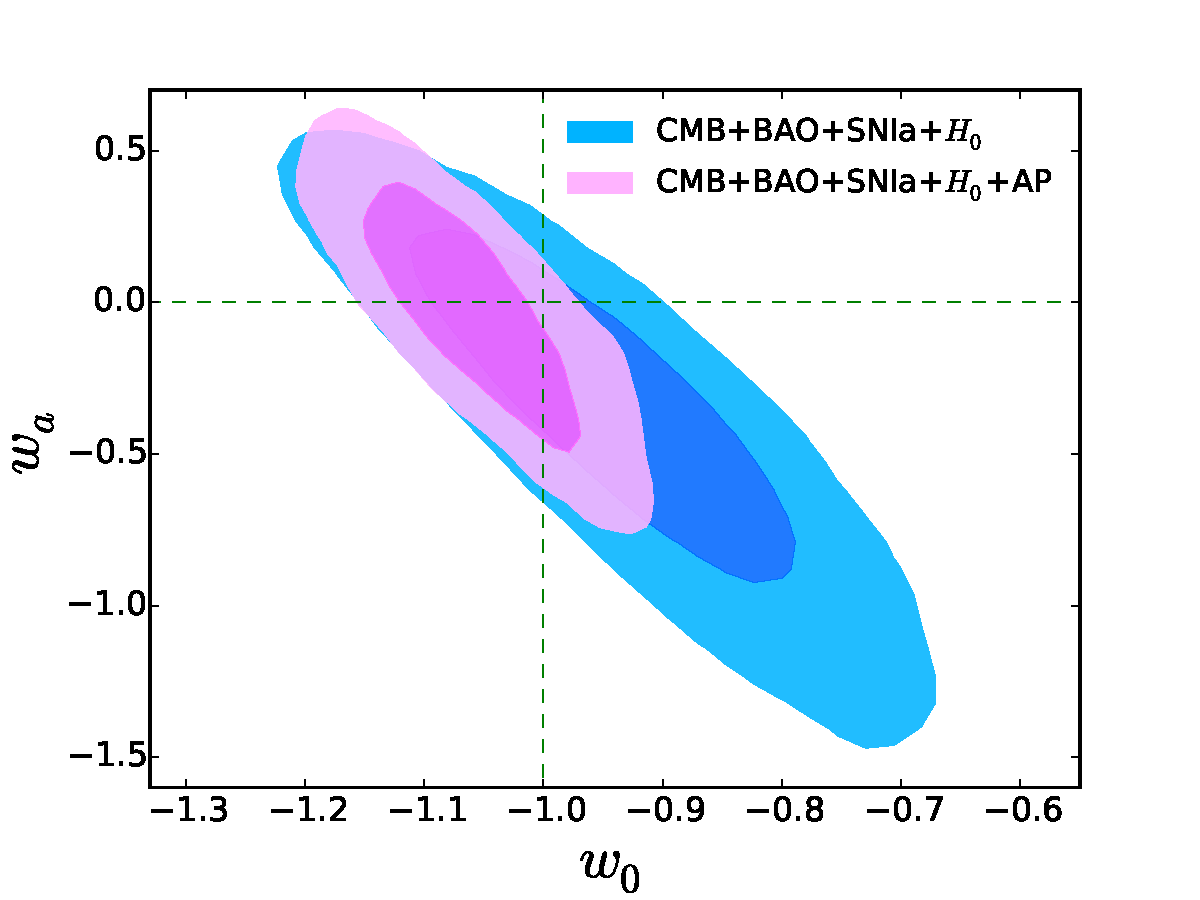
\includegraphics[height=8cm]{fig2b.pdf}
%   \includegraphics[height=8cm]{Tpcf--plot--Normed.eps}
%    \includegraphics[height=8cm]{smu.eps}
   }
   \caption{\label{fig_TpCF}
   Left panel: 68.3\%, 95.4\% CL likelihood contours in the $\Omega_m-w_0$ and $w_0-w_a$ plane.
   Results are consistent with $\Lambda$CDM.
   The constrained area is significantly reduced after adding the AP likelihood.
   This shows the power of the AP method in constraining dynamical dark energy.
   Right panel: Redshift evolution of $w(z)$, with/without adding AP method.
   Adding AP tightens the constraints and reduces the redshift evolution of $w$ (tilt of $w(z)$).
   }
\end{figure*}


\section{Robustness Test}

\citep{Li2016} obtained the constraints on $\Omega_m$ and $w$
\begin{equation}\label{eq:wcdm_constrain_default}
 \Omega_m=0.301\pm 0.006, w=−1.054\pm 0.025.
\end{equation}
Using the technique of ``approximate 2pCF'' and taking a fiducial of $\Omega_m=0.26, w=-1$, we obtains
\begin{equation}
\Omega_m = 0.301 \pm 0.008,\ w=-1.053\pm 0.034\ (\rm fid:\ \Omega_m=0.26, w=-1.0).
%    1  0.3010870E+00  0.7818562E-02  0.2973018E+00  0.3045011E+00  0.2883318E+00  0.3150334E+00   \Omega_m
%    2  0.6886453E+00  0.8507156E-02  0.6802557E+00  0.6975813E+00  0.6708444E+00  0.7047652E+00   h
%    3 -0.1053343E+01  0.3395215E-01 -0.1087474E+01 -0.1020395E+01 -0.1121890E+01 -0.9819443E+00   w
\end{equation}
Since we use smaller $n_{\rm bin}$ than \citep{Li2016}
\footnote{\citep{Li2016} adopted $n_{\rm bin}=25-35$ to achieve tighter constraints.
Since we are using approximate 2pCF, for safty, we use $n_{\rm bin}=20-25$.}, the error bar is slightly larger.
The central values of parameters agree quite well, suggesting the reliability of the approximate 2pCF method.

\begin{figure*}
   \centering{
   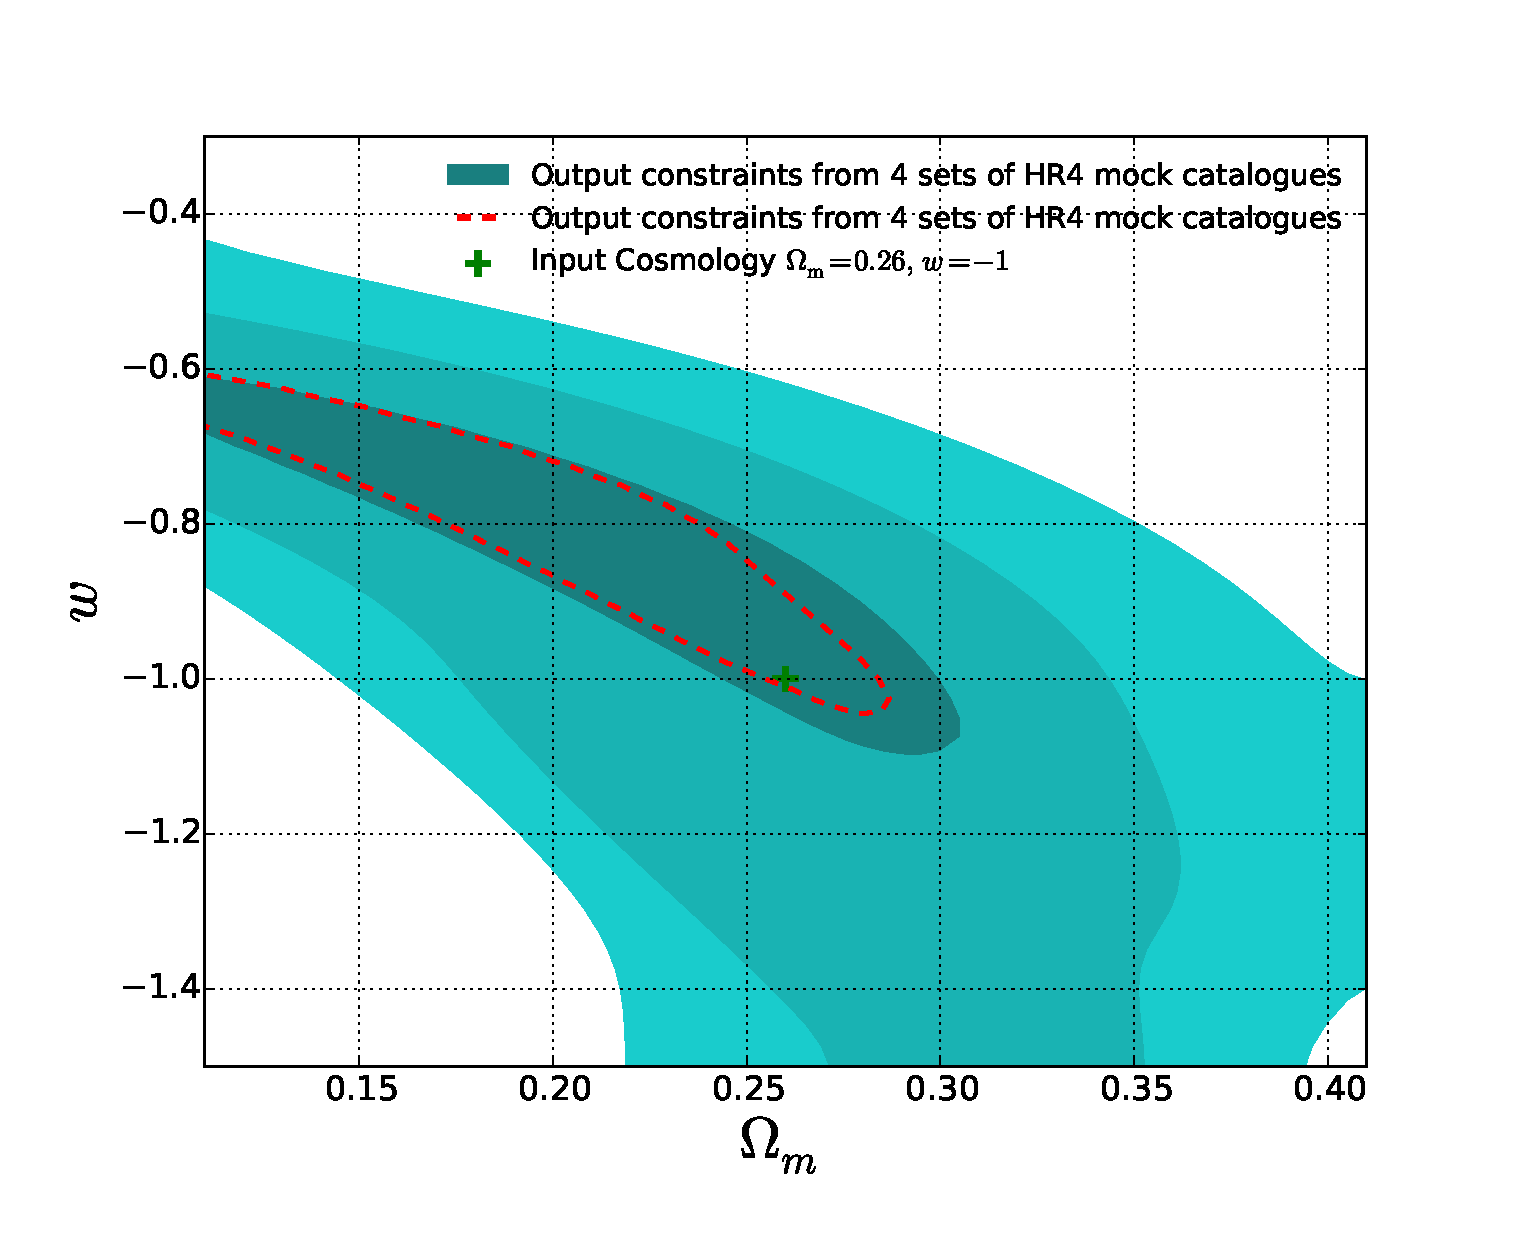
\includegraphics[width=6cm]{figIO.eps}
   %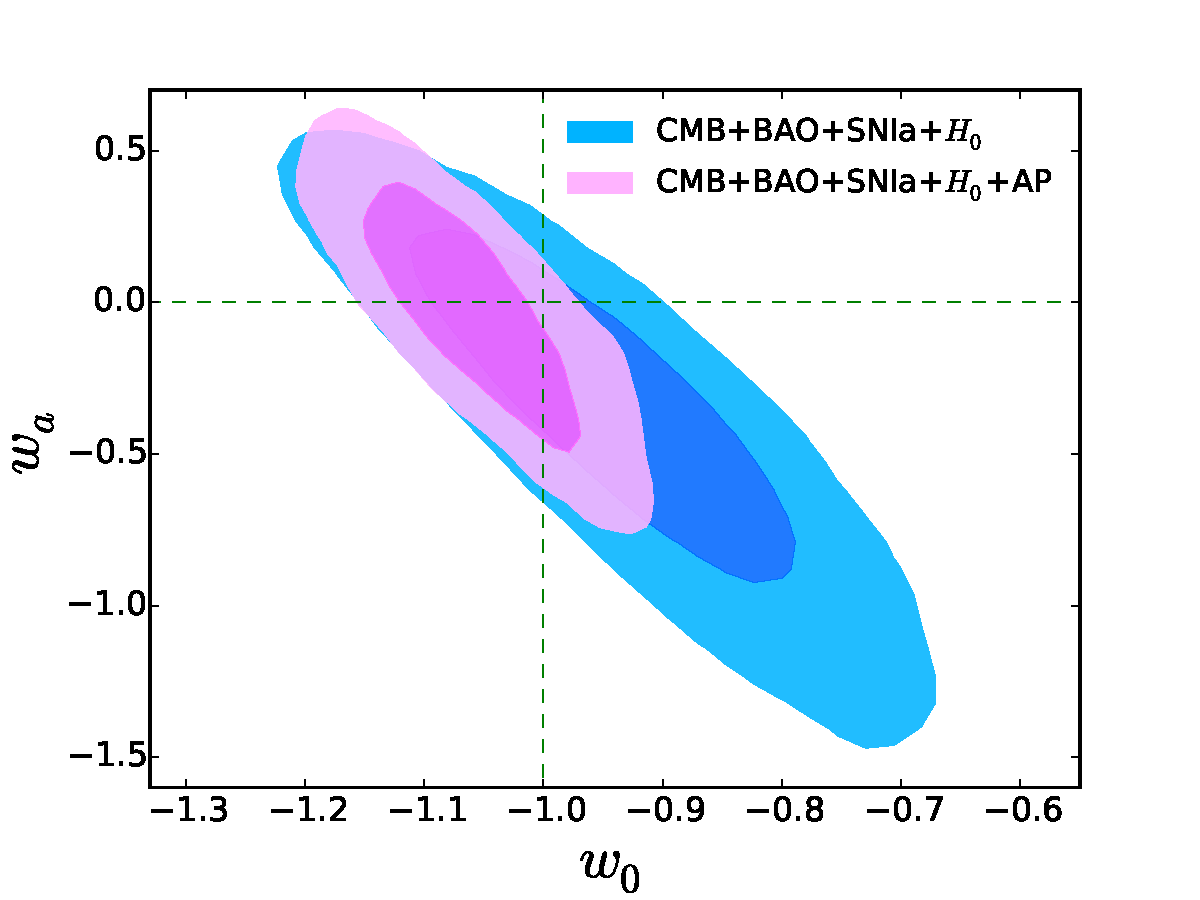
\includegraphics[width=9cm,natwidth=4,natheight=4]{fig2b.pdf}
   %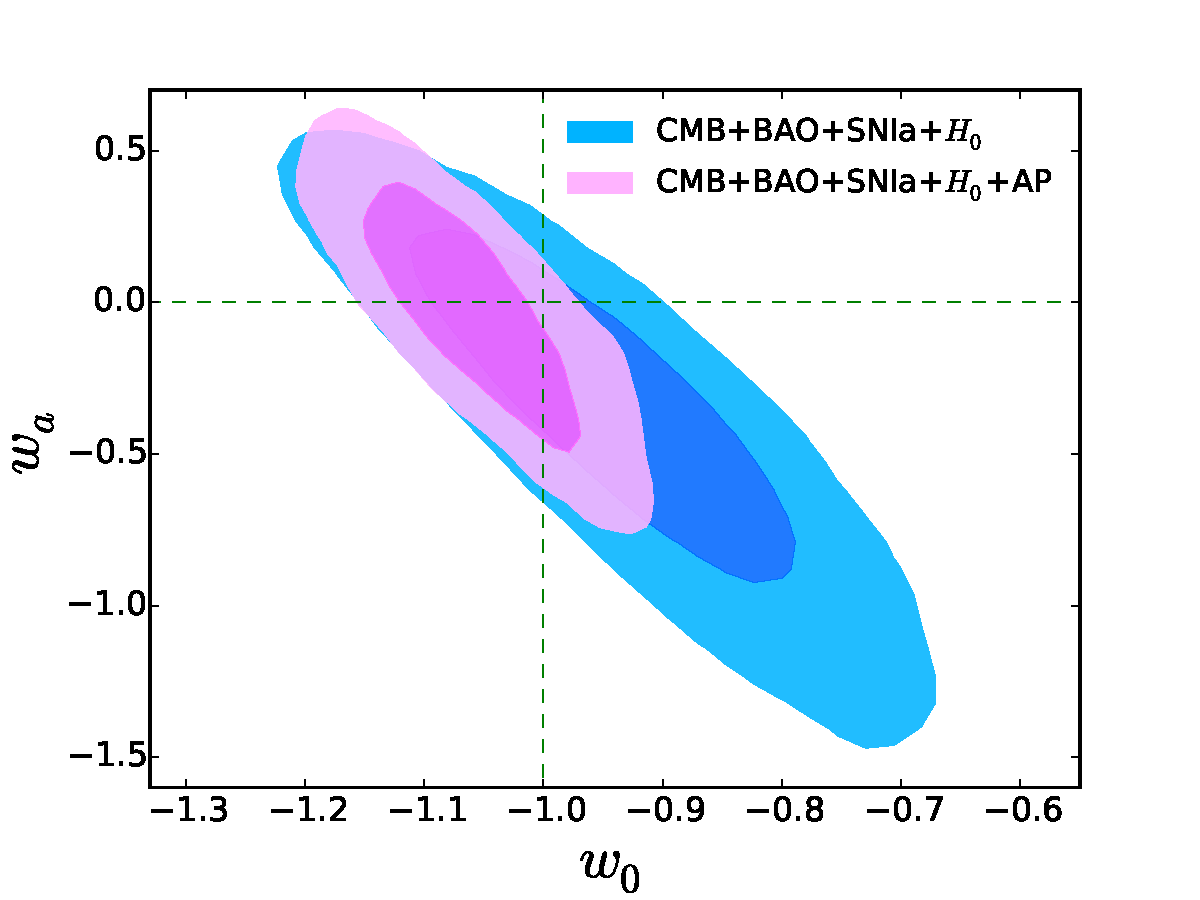
\includegraphics[height=8cm]{fig2b.pdf}
%   \includegraphics[height=8cm]{Tpcf--plot--Normed.eps}
%    \includegraphics[height=8cm]{smu.eps}
   }
   \caption{\label{fig_IO}
   Input-output test of our method.
   }
\end{figure*}

We also did an input-output test on four realizations of HR4 mocks \cite{hr4}.
Figure \ref{fig_IO} shows the input cosmology (marker by green plus) is recovered at $\sim$0.5$\sigma$.

\begin{figure*}
   \centering{
   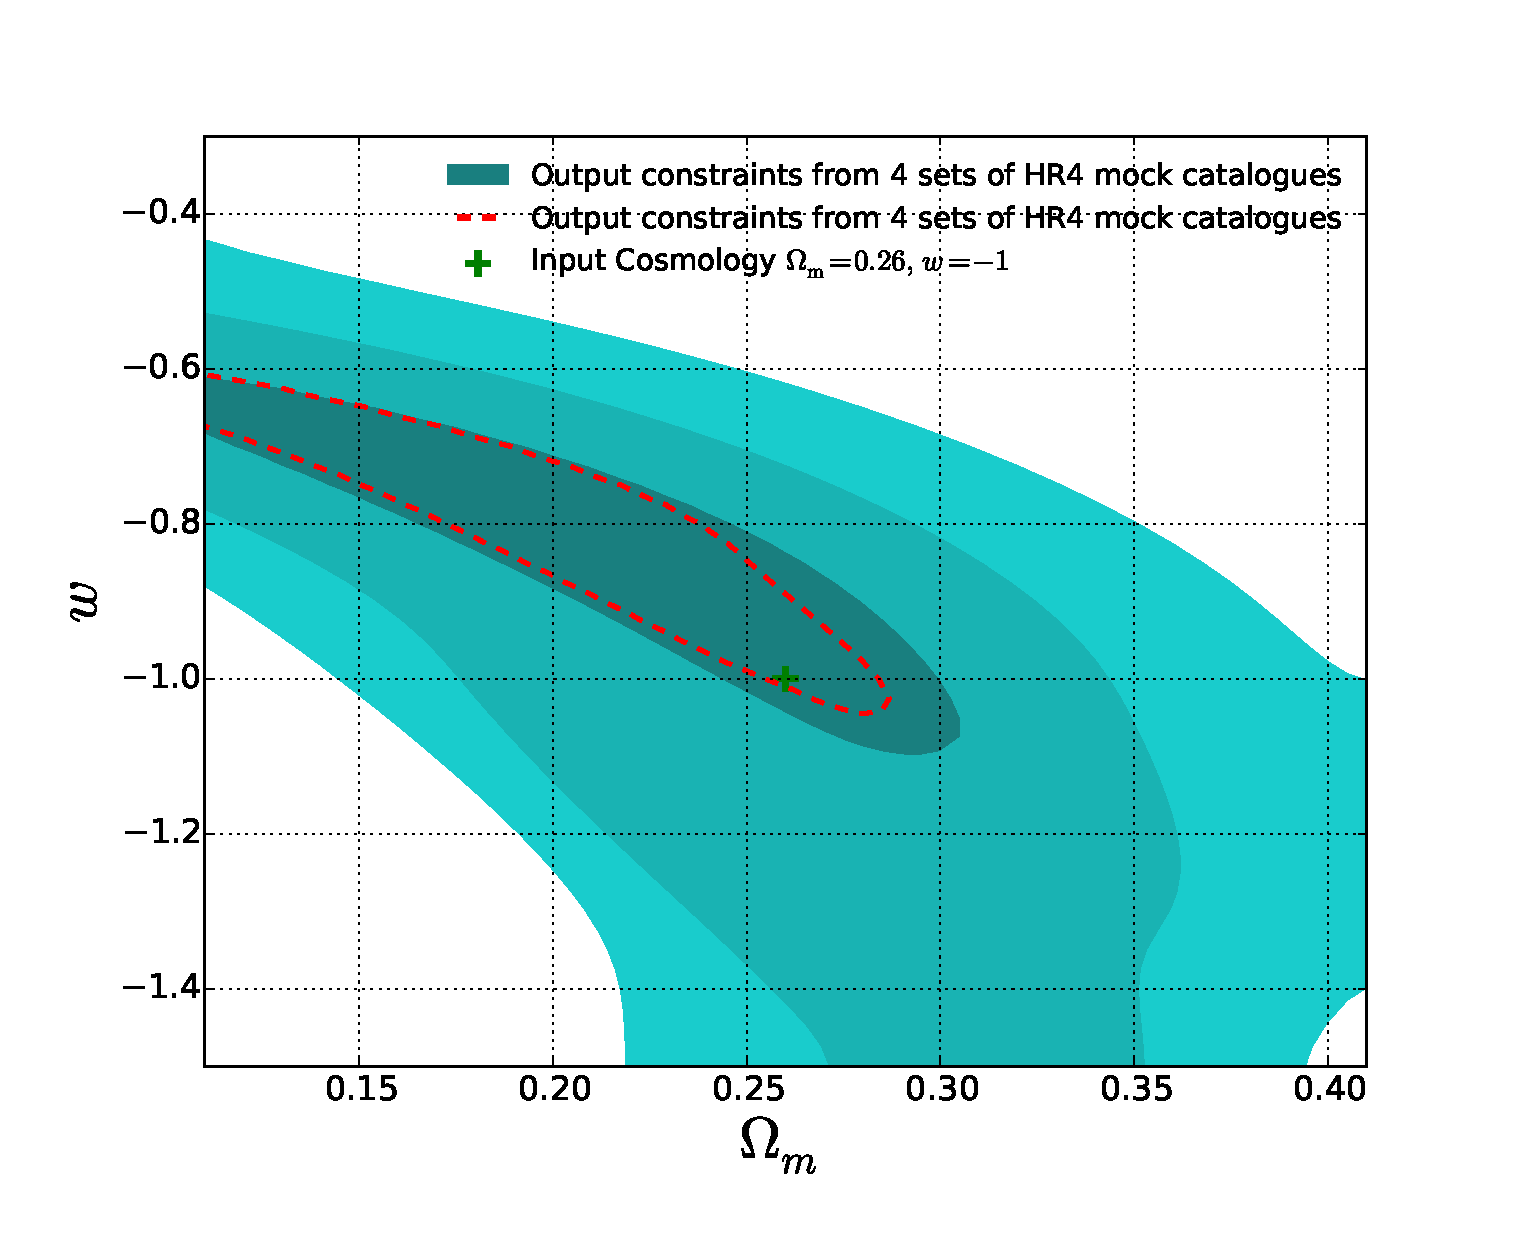
\includegraphics[width=6cm]{figIO.eps}
   %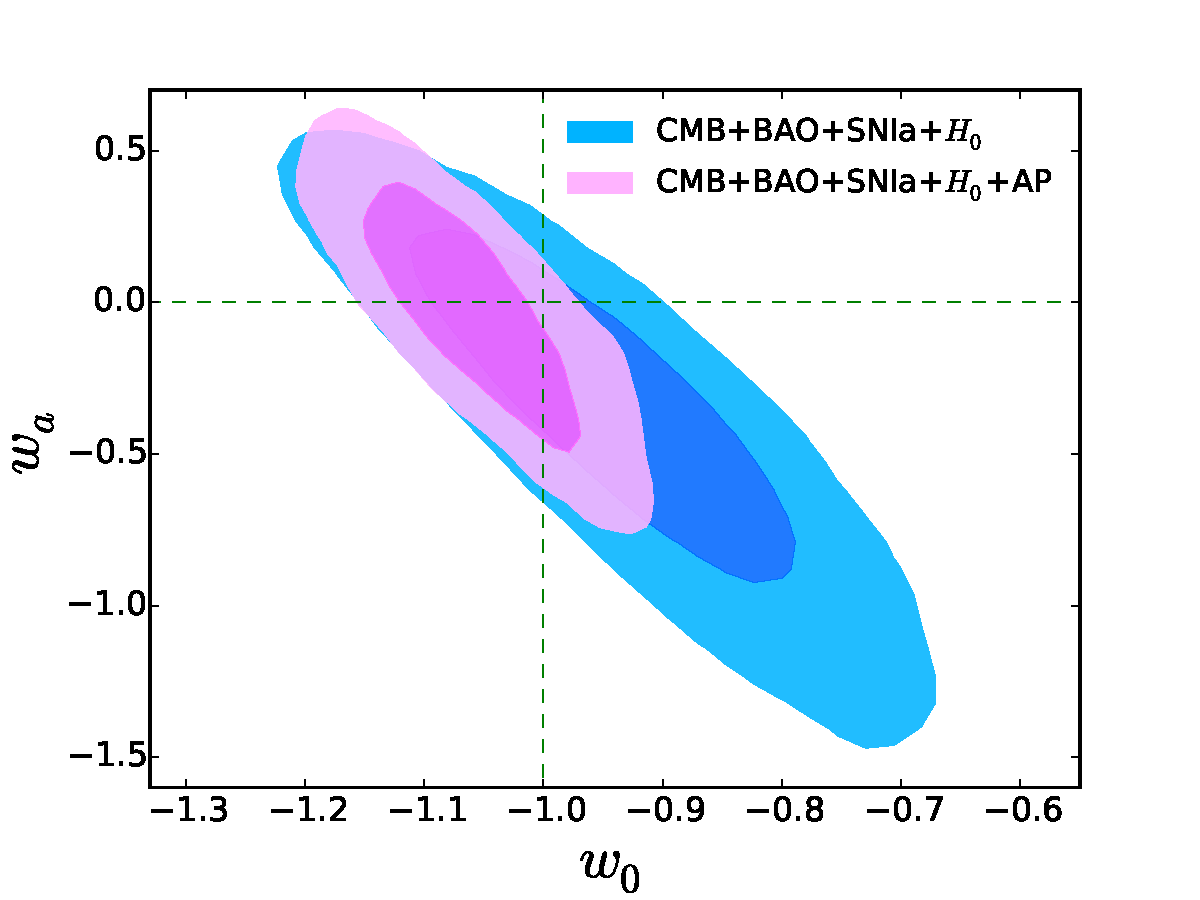
\includegraphics[width=9cm,natwidth=4,natheight=4]{fig2b.pdf}
   %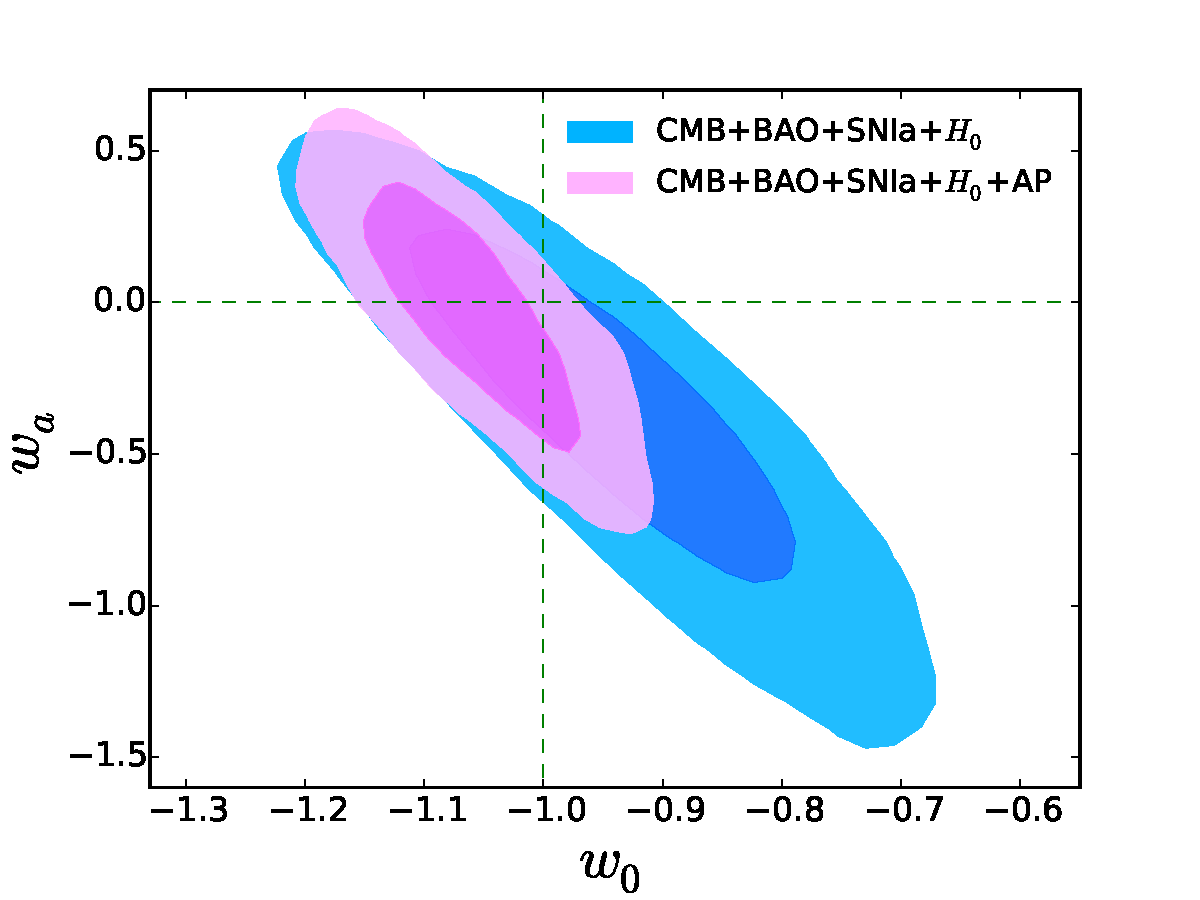
\includegraphics[height=8cm]{fig2b.pdf}
%   \includegraphics[height=8cm]{Tpcf--plot--Normed.eps}
%    \includegraphics[height=8cm]{smu.eps}
   }
   \caption{\label{fig_IO}
   Input-output test of our method.
   }
\end{figure*}

Finally, we did a thourough test of all the our options in our method.
Figure \ref{fig_contest} shows that,
the result almost does not change if 
we adopt $\mu_{\rm max}=0.99\ (0.85)$ to include more (less) near-LOS region in the analysis,
decrease number of bins to $n_{\rm bin}=15-20$,
change the range of clustering to $8-30 \rm Mpc/h$,
change the fiducial cosmology to $\Omega_m=0.26,\ w=-0.6$,
exclude 1 or 2 high redshift bins,
or reduce the number of mocks to 1000.
%Constraints get weaker if increase $s_{\rm min}$,
%but are consistent with the original one.
Even if we choose the fiducial cosmology as a very ridiculous one,
say $\Omega_m=0.11,\ w=-2.0$, the change in contour is still mild.
The very good point is that, 
the shift in contour position is very small if we discard the systematic correction.

%We measure the evolution of $\hat\xi_{\Delta s}$ in six redshift bins.
%on scales of $s_{\rm min}=6$, $s_{\rm max}=40$.
%Systematics subtracted with the help of HR4 simulation.
%Covariance matrix 

\begin{figure*}
   \centering{
   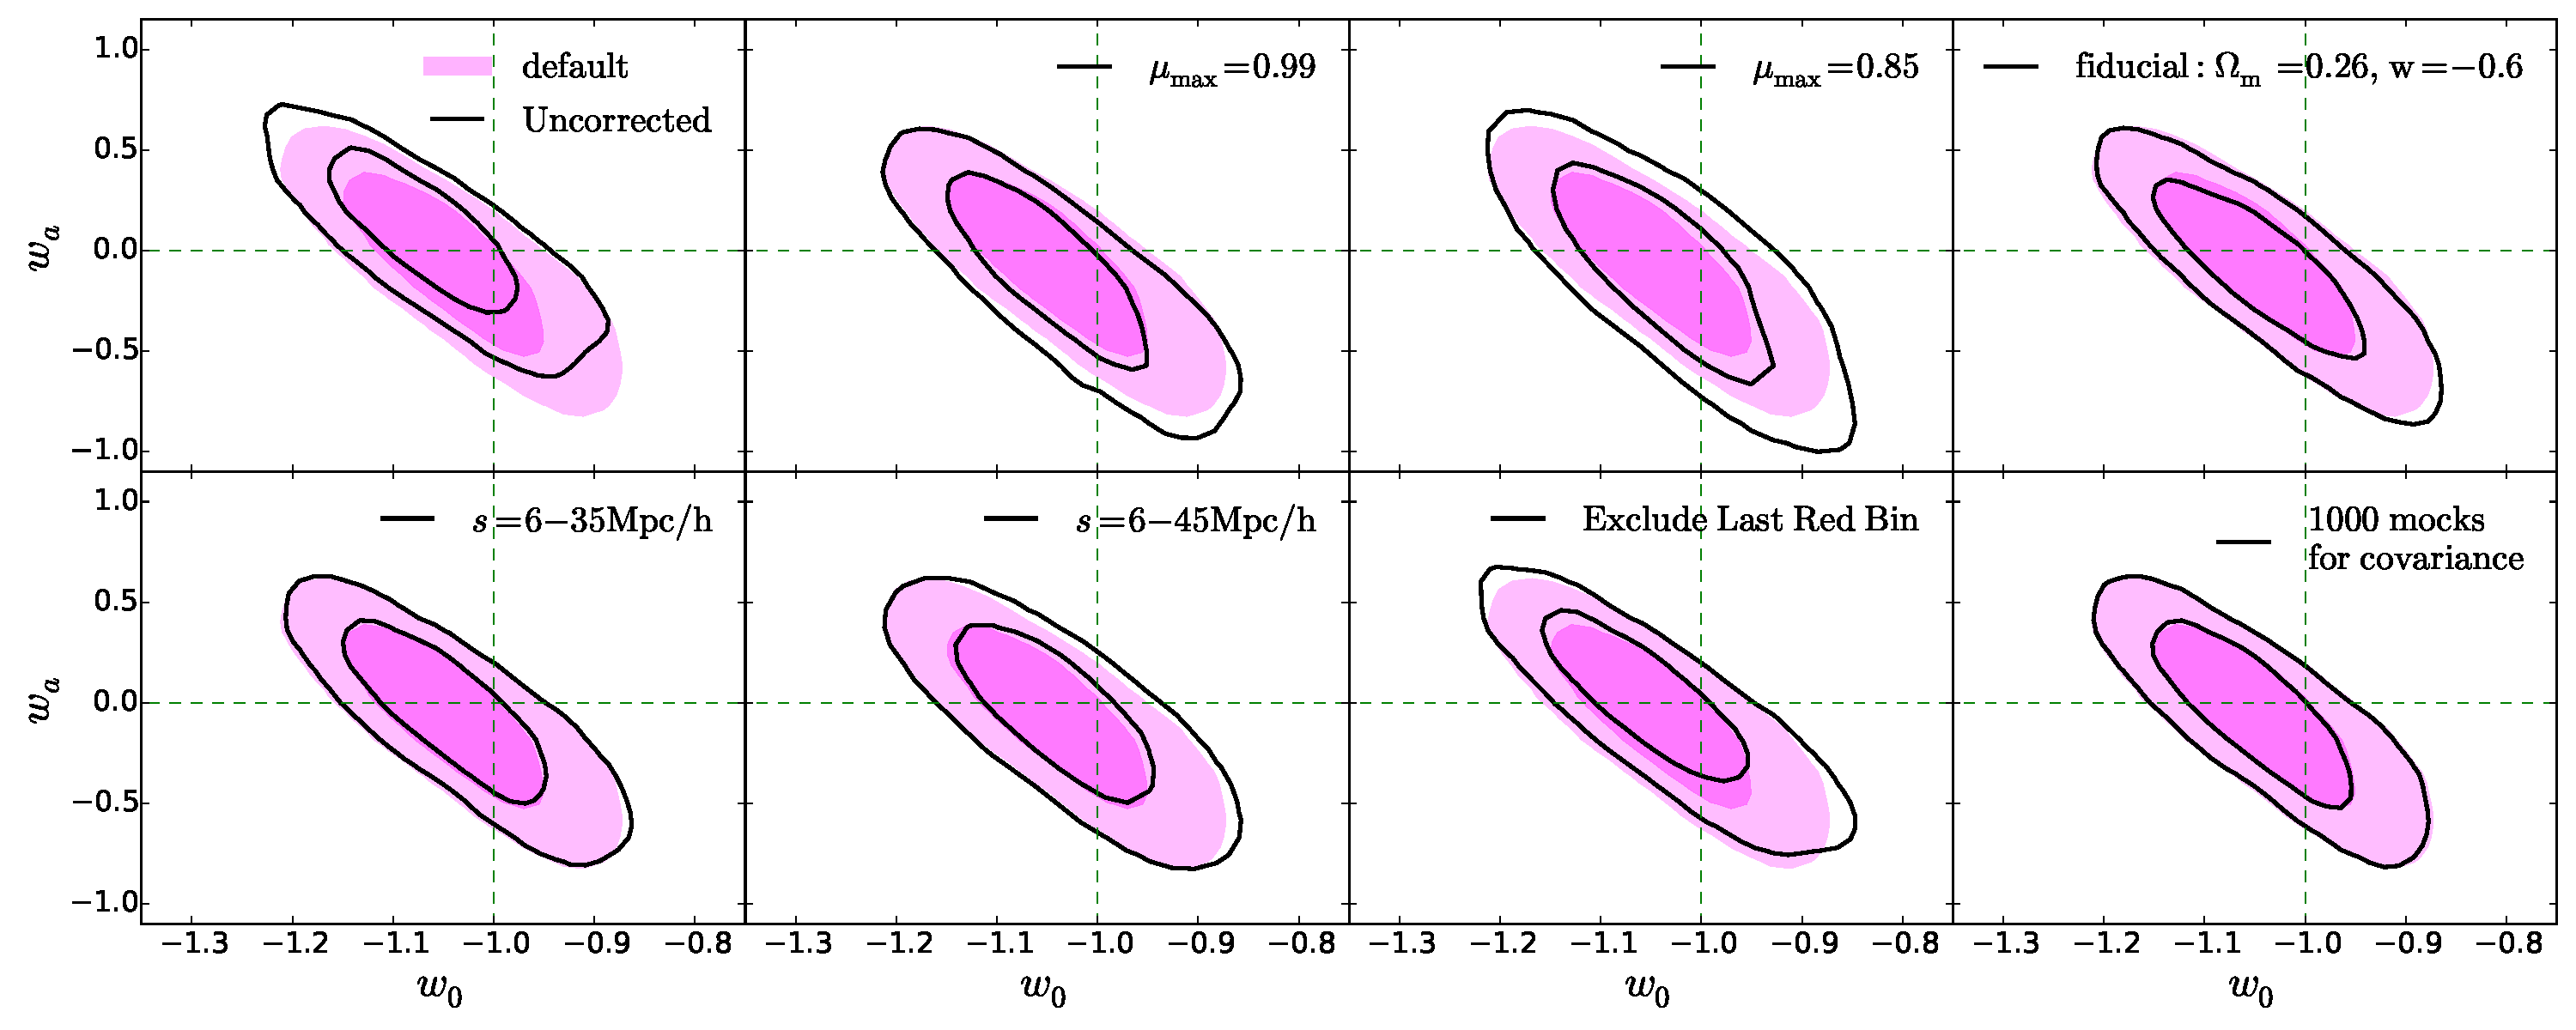
\includegraphics[width=18cm,natwidth=8,natheight=8]{fig_con_tests.pdf}
   %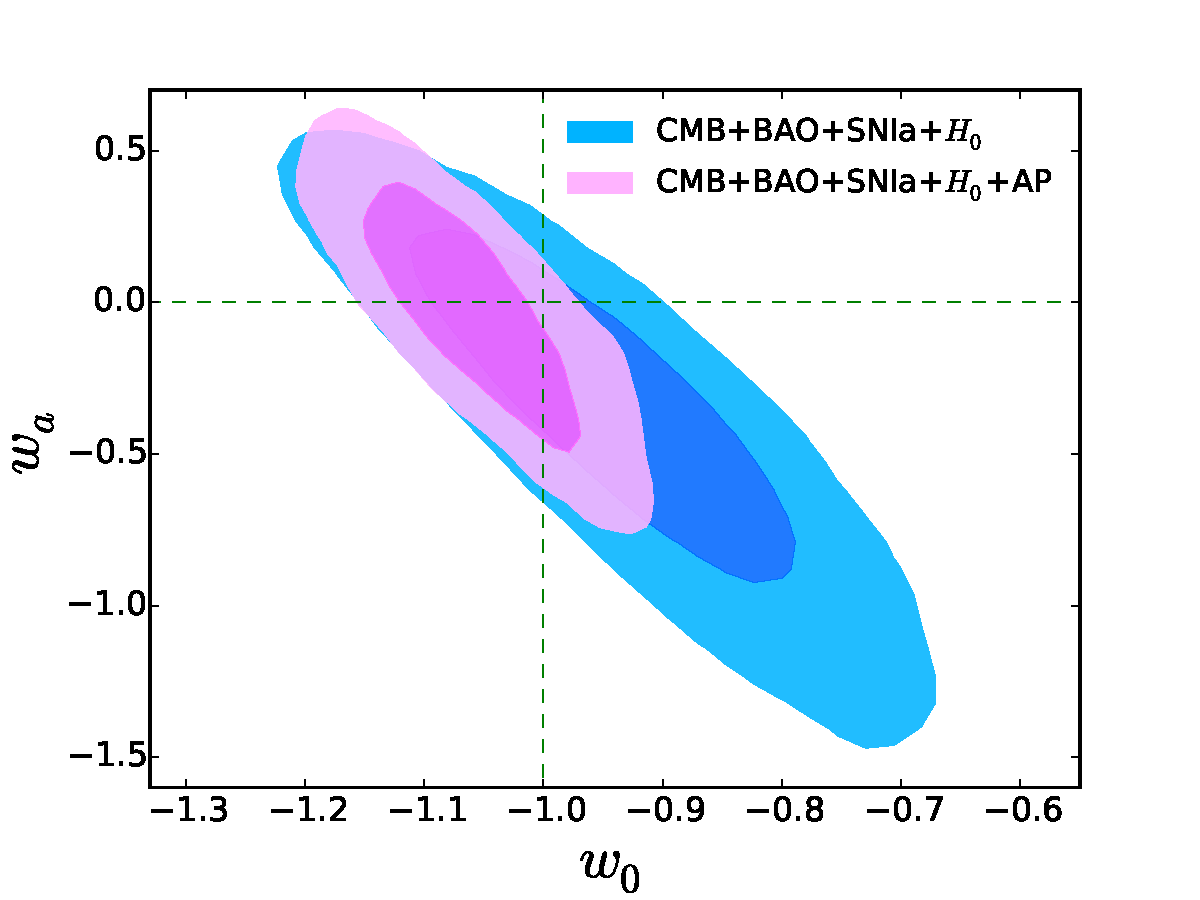
\includegraphics[width=9cm,natwidth=4,natheight=4]{fig2b.pdf}
   %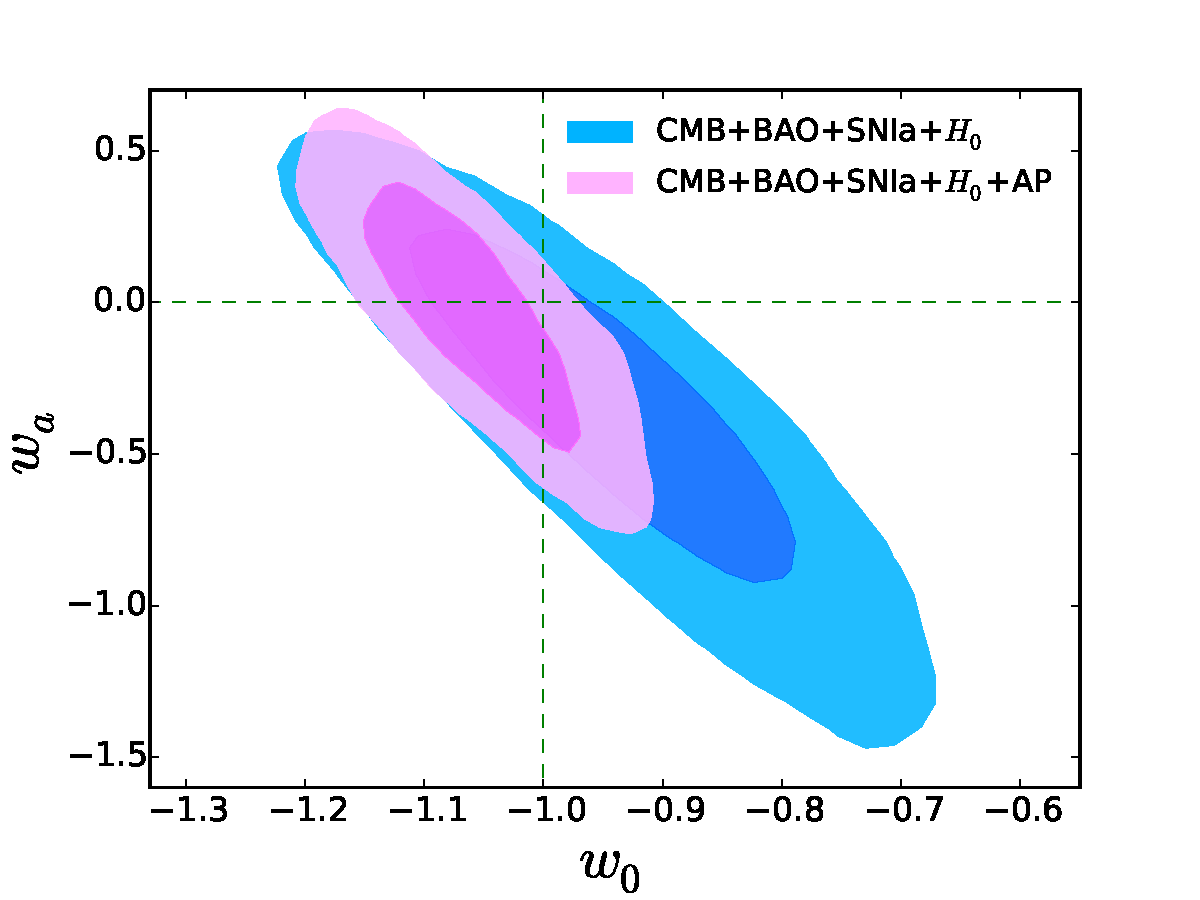
\includegraphics[height=8cm]{fig2b.pdf}
%   \includegraphics[height=8cm]{Tpcf--plot--Normed.eps}
%    \includegraphics[height=8cm]{smu.eps}
   }
   \caption{\label{fig_contest}
   Robustness test of our method.
   }
\end{figure*}

\section{Conclusion}

In \cite{Li2016} we proposed to constrain cosmological parameters via the redshift depence of galaxy clustering.
This enables a robust Alcock-Paczynski test on relatively small scales.
In this paper we improved the methodology and obtained tight constraints of the CPL parametrization.
Adding our method to the CMB+SNIa+BAO+$H_0$ combination, the $w_0-w_a$ contour was reduced by 50\%.

In sum, our AP method have many advantages:
\begin{itemize}
 \item {\it It leads to very tight cosmological constraints (powerful)}. The 
 \item {\it Focusing on the redshift evolution of anisotropy it successfully overcome the problem of RSD, 
 which has long time been a limitation to the application of AP to LSS (successful).}
 In traditional approaches it is very challenging to model the RSD and enable a robust AP test.
 \item {\it It is robust against systematics (reliable)}. 
 \cite{Li2016} shows that $\hat\xi_{\Delta s}$ is insensitive to RSD or galaxy bias.
 Figure \ref{fig_con_tests} shows that the change in results is small even if we do not correct the systematics at all.
 \item {\it It is a major advance in extracting cosmological information on relatively small scales clustering (unique).} 
 Clustering of galaxies happen on all scales,
but the size and shape of BAO ring only captures information mostly on scales of $s=100-120 {\rm Mpc/h}$.
In the analysis of correlation function shape, people mostly use $s\gtrsim 40$ Mpc/h.
Our AP method enters much smaller scales.
%Actually, there are more structures formed on smaller scales.
%Surely cosmologists should find one method to $reliably$ utilize these scales.
%Our method could be one solution.
 \item {\it It does not require complicate modeling of non-linear structure growth and RSD (simple).}
 \item {\it It is complimentary to BAO (useful).}
 The method explores much smaller clustering scales than BAO. 
 \cite{Li2016} shows that, actually the directions of $\Omega_m-w$ contours of the two methods are orthogonal to each other.
\end{itemize}


While it is of essential importance to build larger experiments to 
explore more of our Universe,
the physical interpration of the data is of equal importance.
Considering our method enables {\it twice as much as before} information about the cosmic expansion history extracted from LSS data.
This, in a way, significantly enhances the valuable data obtained from the very expensive experiments costing billions of dollars.

The method can be applied to many future spectroscopic surveys. 
We expect it play an important role in in helping us unveiling the dark energy.






\section*{Acknowledgments}

We thank the Korea Institute for Advanced Study for providing computing resources (KIAS Center for Advanced Computation Linux Cluster System).
We thank Seokcheon Lee and Graziano Rossi for many helpful discussions.


\begin{thebibliography}{}


\bibitem[Ade et al. (2015)]{Planck2015}
Ade, P.A.R., Aghanim, N., \& Arnaud, M., et al. arXiv:1502.01589

\bibitem[Alam et al.(2016)]{Alam2016}
Alam, S., Ata, M., \& Bailey, S., et al. 2016,
submitted to MNRAS (arXiv:1607.03155)

\bibitem[{{Alam} {et~al}\mbox{.}(2015{\natexlab{a}}){Alam}, {Albareti},
  {Allende Prieto}, {Anders}, {Anderson}, {Anderton}, {Andrews}, {Armengaud},
  {Aubourg}, {Bailey}, \& et~al.}]{dr12}
{Alam} S., Albareti, F.D.,\& Allende Prieto, C., {et~al.}, 2015,  ApJS, 219, 12

\bibitem[Alcock \& Paczynski(1979)]{AP1979}
Alcock, C., \& Paczynski, B. 1979, Nature, 281, 358  

%\bibitem[Anderson et al.(2012)]{2012MNRAS.427.3435A} 
%Anderson, L., Aubourg, E., Bailey, S., et al.\ 2012, MNRAS, 427, 3435

\bibitem[Anderson et al.(2013)]{Anderson2013}
Anderson, L., Aubourg, \'E., \& Bailey, S. et al. 2014, MNRAS, 441, 24  
  
%\bibitem[Bassett et al.(2002)]{Bassett2002}
%Bassett, B.A., Kunz, M., Silk, J., \& Ungarelli, C. 2002, MNRAS, 336, 1217

\bibitem[Ballinger, Peacock \& Heavens 1996]{Ballinger1996}
Ballinger, W.E., Peacock, J.A., \& Heavens, A.F. 1996, MNRAS, 282, 877  

\bibitem[Betoule et al.(2014)]{JLA}
Betoule, M., Kessler, R., \& Guy, J., et al. 2014, A\&A, 568, 32


\bibitem[Beutler et al.(2011)]{6dFGS}
Beutler, F., Blake, C., \& Colless, M., et al. 2011, MNRAS, 416, 3017

\bibitem[Beutler et al.(2013)]{Beutler2013}
Beutler, F., Saito, S., \& Seo, H.-J., et al. 2013, MNRAS, 443, 1065

\bibitem[Beutler et al.(2016)]{Beutler2016}
Beutler, F., Seo, H.-J., \& Saito, S., et al. 2016,
arXiv:1607.03150

\bibitem[Blake et al.(2011)]{Blake2011}
Blake, C., Glazebrook, K., \& Davis, T. M., 2011, MNRAS, 418, 1725  

\bibitem[Blake et al.(2013)]{WiggleZtopoloy}
Blake, C., James, J.B., \& Poole, G.B. 2013, MNRAS, 437, 2488

\bibitem[Bolton et al.(2012)]{Bolton2012}
Bolton, A.S., Schlegel, \& D.J., Aubourg E., et al. 2012, AJ, 144, 144

\bibitem[Boylan-Kolchin et al.(2008)]{B08}
Boylan-Kolchin, M., Ma, C.-P., \& Quataert, E. 2008, MNRAS, 383, 93


%\bibitem[Bueno Belloso et al. (2012)]{BB2012}
%Bueno Belloso, A., Pettinari, G.W., Meures, N., \& Percival, W.J. 2012, Phys. Rev. D, 86, 023530

%\bibitem[Chevallier \& Polarski(2001)]{CP2001}
%Chevallier, M., Polarski, D. 2001, Int. J. Mod. Phys. D, 10, 213


%\bibitem[Choi et al.(2010)]{choi 2010}
%Choi, Y.-Y., Park, C., Kim, J., Gott, J.R., 
%Weinberg, D.H., Vogeley, M.S., \& Kim, S.S. 2010, ApJS, 190, 181

\bibitem[Christensen et al.(2001)]{Bayesian}
Christensen, N., Meyer, R., Knox, L., \& Luey, B. 2001, Class. Quant. Grav., 18, 2677

%\bibitem[Chuang et al.(2013)]{Chuang2013}
%Chuang, C.-H., Prada, F., Beutler, F., et al. 2013, arXiv:1312.4889  

\bibitem[Chuang \& Wang(2012)]{ChuangWang2012}
Chuang, C.-H., \& Wang, Y. 2012, MNRAS, 426, 226  


%\bibitem[Corasaniti \& Copeland(2003)]{Corasaniti2003}
%Corasaniti, P.S., Copeland, E.J. 2003, Phys. Rev. D, 67, 063521

%eBOSS: 
%http://arxiv.org/abs/1508.04473
\bibitem[Dawson et al.(2015)]{eBOSS}
Dawson, K.S., Kneib, J.P., \& Percival, W.J., et al. 2015, accepted AJ

\bibitem[Dawson et al.(2012)]{Dawson et al. 2012}
Dawson, K.S., Schlegel, D.J., \& Ahn, C.P., et al. 2012, AJ, 145, 10

\bibitem[Efstathiou (2014)]{E14H0}
Efstathiou, G. 2014, MNRAS, 440, 1138

\bibitem[Eisenstein et al.(2011)]{Eisenstein et al. 2011}
Eisenstein, D.J.,  Weinberg, D.H., \& Agolet, E., et al. 2011, AJ, 142, 72

\bibitem[Feldman, Kaiser \& Peacock (1994)]{1994ApJ...426...23F} 
Feldman, H.A., Kaiser, N., \& Peacock, J.A.\ 1994, ApJ, 426, 23 

\bibitem[Fukugita et al. (1996)]{Fukugita1996}
Fukugita, M., Ichikawa, T., \& Gunn, J.E., et al. 1996, AJ, 111, 1748
%Publication:	
%Astronomical Journal v.111, p.1748 

%\bibitem[Gingold \& Monaghan(1977)]{GM1977}
%Gingold, R.A., \& Monaghan, J.J. 1977, MNRAS, 181, 375  

%\bibitem[Gott et al.(2009)]{gott 2009}
%Gott, J.R., Choi, Y.-Y., Park, C., \& Kim, J. 2009, ApJ, 695, L45  

%\bibitem[Gott et al.(2008)]{gott 2008}
%Gott, J.R., Hambrick, D.C., Vogeley, M.S., Kim, J., Park, C., Choi, Y.-Y.,
%Cen, R., Ostriker, J.P., \& Nagamine, K. 2008, ApJ, 675, 16  


\bibitem[Gunn et al. (1998)]{Gunn1998}	
Gunn, J.E., Carr, M., \& Rockosi, C. et al. 1998, AJ, 116, 3040

\bibitem[Gunn et al.(2006)]{Gunn et al. 2006}
Gunn, J.E., Siegmund, W.A., \& Mannery, E.J., et al. 2006, AJ, 131, 2332

\bibitem[Guzzo et al.(2008)]{Guzzo2008}
Guzzo, L., Pierleoni, M., \& Meneux, B., et al. 2008, Nature, 451, 541

\bibitem[Hartlap et al.(2006)]{Hartlap}
Hartlap J., Simon P. \& Schneider P. [astro-ph/0608064].


\bibitem[Hong et al.(2016)]{hong2016}
Hong, S.E., Park, C.,\&  Kim, J. 2016, ApJ, 823, 103

\bibitem[Jackson (1972)]{FOG}
Jackson, J., 1972, MNRAS, 156, 1

\bibitem[Jennings et al.(2011)]{Jennings2011}
Jennings, E., Baugh, C.M., \& Pascoli, S. 2011, MNRAS, 420, 1079  

%\bibitem[Jeong et al.(2014)]{Jeong2014}
%Jeong, D., Dai, L., Kamionkowski, M., \& Szalay, A.S. 2014, arXiv:1408.4648

\bibitem[Jiang et al.(2008)]{jiang2008}
Jiang, C.Y., Jing, Y. P., \& Faltenbacher, A., et al. 2008, ApJ, 675, 1095

\bibitem[Kaiser (1987)]{Kaiser1987}
Kaiser, N. 1987, MNRAS, 227, 1


\bibitem[Kim \& Park(2006)]{kim and park 2006}
Kim, J., \& Park, C. 2006, ApJ, 639, 600  

\bibitem[Kim et al.(2009)]{2009ApJ...701.1547K} 
Kim, J., Park, C., Gott, J.R., III, \& Dubinski, J.\ 2009, ApJ, 701, 1547 

\bibitem[Kim et al.(2015)]{hr4}
Kim, J., Park, C., L'Huillier, B., \& Hong, S. E. 2015, JKAS, 48, 213

\bibitem[Kim et al.(2011)]{horizonrun}
Kim, J., Park, C., Rossi, G., Lee, S.M., \& Gott, J.R. 2011, JKAS, 44, 217  

\bibitem[Kitaura et al.(2015)]{MDPATCHY}
Kitaura, F.S., Rodrı\'{i}guez-Torres, S., Chuang, C.-H., et al. arXiv:1509.06400

\bibitem[Komatsu et al.(2011)]{komatsu 2011}
Komatsu, E., Smith, K. M., \& Dunkley, J., et al. 2011, ApJS, 192, 18  

\bibitem[Lacey \& Cole(1993)]{LC93}
Lacey, C., \& Cole, S. 1993, MNRAS, 262, 627


\bibitem[Landy \& Szalay(1993)]{1993ApJ...412...64L} 
Landy, S.D., \& Szalay, A.S.\ 1993, ApJ, 412, 64 

%EUCLID:
%http://arxiv.org/abs/1110.3193
\bibitem[Laureijs et al.(2011)]{EUCLID}
Laureijs, R., Amiaux, J., \& Arduini, S., et al. 2011, arXiv:1110.3193

\bibitem[Lavaux \& Wandelt(2012)]{LavausWandelt1995}
Lavaux, G., \& Wandelt, B.D. 2012, ApJ, 754, 109  

%\bibitem[Levi et al.(2013)]{2013arXiv1308.0847L} 
%Levi, M., Bebek, C., Beers, T., et al.\ 2013, arXiv:1308.0847 

\bibitem[Lewis \& Bridle (2002)]{LB2002}
Lewis, A., \& Bridle, S. 2002, Phys. Rev. D, 66, 103511

\bibitem[L'Huillier et al.(2014)]{2014NewA...30...79L} 
L'Huillier, B., Park, C., \& Kim, J.\ 2014, New Astronomy, 30, 79 

\bibitem[Li et al.(2011)]{Li2011}
Li, M., Li, X.-D., Wang, S., \& Wang, Y. 2011, Commun. Theor. Phys., 56, 525

\bibitem[Li et al.(2014)]{Li2014}
Li, X.-D., Park, C., Forero-Romero, J., \& Kim, J. 2014, ApJ, 796, 137

\bibitem[Li et al.(2015)]{Li2015}
Li, X.-D., Park, C., Sabiu, C.G., \& Kim, J. 2015, MNRAS, 450, 807 

\bibitem[Li et al.(2015)]{Li2016}
Li, X.-D., Park, C., Sabiu, C.G., \& Kim, J. 2015, MNRAS, 450, 807 

%\bibitem[Linder(2003)]{Linder2003}
%Linder, E.V. 2003, Phys. Rev. Lett., 90, 091301

\bibitem[Linder et al.(2014)]{Linder2013}
Linder, E.V., Minji, O., Okumura, T., Sabiu, C.G., \& Song, Y.-S. 2014, Phys. Rev. D, 89, 063525  

\bibitem[L{\'o}pez-Corredoira(2014)]{2014ApJ...781...96L} 
L{\'o}pez-Corredoira, M.\ 2014, ApJ, 781, 96 

\bibitem[Mao et al. (2016)]{Qingqing2016}
Mao, Q., Berlind, A.A., Scherrer, R.J., et al. 2016, submitted to ApJ

\bibitem[Marinoni \& Buzzi(2010)]{Marinoni2010}
Marinoni, C., \& Buzzi, A. 2010, Nature, 468, 539  

\bibitem[Matsubara \& Suto(1996)]{Matsubara1996}
Matsubara T., \& Suto, Y. 1996, ApJ, 470, L1  

\bibitem[McCavana et al.(2012)]{M12}
McCavana, T., Micic, M., Lewis, G. F., et al. 2012, MNRAS, 424, 361


\bibitem[Morandi \& Sun (2016)]{MS2016}
Morandi, A., \& Sun, M. arXiv:1601.03741


\bibitem[Outram et al.(2004)]{Outram2004}
Outram, P.J., Shanks, T., Boyle, B.J., Croom, S.M., Hoyle, F., Loaring, N.S., 
Miller, L., \& Smith, R.J. 2004, MNRAS, 348, 745  

%\bibitem[Parejko et al.(2013)]{Parejko2013}
%Parejko, J. K., Sunayama, T., Padmanabhan, N., et al. 2013, MNRAS, 429, 98  

\bibitem[Parejko et al.(2013)]{Parejko2013}
Parejko J.K., et al., 2013, MNRAS, 429, 98

\bibitem[Parihar et al. (2014)]{CMASSLSS2014}
Parihar, P., Vogeley, M.S., \& Gott, J.R., et al. 2014, ApJ, 796, 86

\bibitem[Park et al.(2005)]{park 2005}
Park, C., Kim, J., \& Gott, J.R. 2005, ApJ, 633, 1  

\bibitem[Park \& Kim(2010)]{topology}
Park, C., \& Kim, Y.-R. 2010, ApJL, 715, L185  

\bibitem[Park et al. (2012)]{Park2012}
Park, C., Choi, Y.-Y., Kim, J., Gott, J.R., Kim, S.S., \&
Kim, K.-S. 2012, ApJ, 759, 7

\bibitem[Park et al. (2015)]{Park2015}
Park, C., Song, H., Einasto, M., Lietzen, H., \&
Heinamaki, P. 2015, JKAS, 48, 75

\bibitem[Peebles \& Ratra(2003)]{PR2003}
Peebles, P.J.E., \& Ratra, B. 2003, Reviews of Modern Physics, 75, 559

\bibitem[Percival et al.(2014)]{Percival2014}
Percival, W.J., Ross, A.J., \& S\'{a}nchez, A.G., et al. 2014, MNRAS, 439, 2531

\bibitem[Perlmutter et al.(1999)]{Perl1999}
Perlmutter, S., Aldering, G., \& Goldhaber, G., et al. 1999, ApJ, 517, 565  

\bibitem[Press \& Shechter(1974)]{PS1974}
Press, W.H., \& Schechter, P.L. 1974, ApJ, 187, 425



\bibitem[Reid et al.(2012)]{Reid2012}
Reid, B., Samushia, L., \& White, M., et al. 2012, MNRAS, 426, 2719  

\bibitem[Reid et al.(2016)]{Reidetal:2016}
Reid, B., Ho, S., \& Padmanabhan, N., et al.  2016, MNRAS, 455, 1553

\bibitem[Riess et al.(1998)]{Riess1998}
Riess, A.G., Filippenko, A.V., \& Challis, P., et al. 1998, AJ, 116, 1009  

\bibitem[Riess et al.(2011)]{Riess2011}
Riess, A.G., Macri, L., \& Casertano, S., et al. 2011, ApJ, 730, 119
%A 3\% Solution: Determination of the Hubble Constant with the Hubble Space Telescope and Wide Field Camera

\bibitem[Ross et al.(2012)]{2012MNRAS.424..564R} 
Ross, A.J., Percival, W.J., \& S{\'a}nchez, A.G. et al.\ 2012, MNRAS, 424, 564 

\bibitem[Ross et al.(2015)]{MGS}
Ross, A.J., Samushia, L., \& Howlett, C., et al. 2015, MNRAS, 449, 835

\bibitem[Ryden(1995)]{Ryden1995}
Ryden, B.S. 1995, ApJ, 452, 25  

%\bibitem[Samushia et al.(2014)]{Samushia2014}
%Samushia, L., Reid, B. A., White, M., et al. 2014, MNRAS, 439, 3504  

%\bibitem[Sanchez et al.(2013)]{Sanchez2013}
%Sanchez, A. G., Kazin, E. A., Beutler, F., et al. 2013, MNRAS, 433, 1202  

%\bibitem[Sutter et al.(2014)]{Sutter2014}
%Sutter, P.M., Pisani, A., Wandelt, B.D., \& Weinberg, D.H. 2014, MNRAS, 443, 2983


\bibitem[Sanchez et al.(2016)]{Sanchez2016}
Sanchez, A. G., Scoccimarro, R., \& Crocce, M., et al.
arXiv:1607.03147

\bibitem[Schlafly et al.(2010)]{Schlafly2010}
Schlafly E.F., Finkbeiner D.P., Schlegel D.J., et al. 2010, ApJ, 725, 1175

\bibitem[Schlafly \& Finkbeiner(2011)]{SF2011}
Schlafly E.F., \& Finkbeiner D.P. 2011, ApJ, 737, 103


%DESI:
%http://arxiv.org/abs/1106.1706
\bibitem[Schlegel et al.(2011)]{DESI}
Schlegel, D., Abdalla, F., \& Abraham, T., et al. 2011, arXiv:1106.1706

\bibitem[Smee et al.(2013)]{Smee2013}
Smee, S.A., Gunn, J.E., \& Uomoto, A., et al. 2013, AJ, 146, 32

\bibitem[Song et al.(2014)]{2014arXiv1407.2257S} 
Song, Y.S., Sabiu, C.G., 
Okumura, T., Oh, M., \& Linder, E.V.\ 2014, JCAP, 12, 005 

\bibitem[Speare et al. (2015)]{Speare2015}
Speare, R., Gott, J.R., Kim, J., \& Park, C.
2015, ApJ, 799, 176

%\bibitem[Tojeiro \& Percival(2011)]{Tojeiro2011}
%Tojeiro R., \& Percivial W.J. 2011, MNRAS, 417, 1114  

%\bibitem[Tojeiro et al.(2012)]{Tojeiro2012}
%Tojeiro, R., Percival, W. J., Wake, D. A., et al. 2012, MNRAS, 424, 136 

\bibitem[Viana \& Liddle(1996)]{VL1996}
Viana, P.T.P., \& Liddle, A.R. 1996, MNRAS, 281, 323

\bibitem[Villalobos et al.(2013)]{V13}
Villalobos, \'{A}., ́De Lucia, G., Weinmann, S.M., Borgani, S., \& Murante, G. 2013, MNRAS, 433, L49


\bibitem[Weinberg (1989)]{SW1989}
Weinberg, S. 1989, Reviews of Modern Physics, 61, 1

\bibitem[White (2011)]{White2011}
White M., et al. 2011, ApJ, 728, 126

\bibitem[York et al.(2000)]{York et al. 2000}
York, D.G., Adelman, J., \& Anderson, J.E., et al. 2000, AJ, 120, 1579

\bibitem[Zehavi et al.(2011)]{zehavi2011}
Zehavi, I., Zheng, Z., \& Weinberg, D.H., et al. 2011, ApJ, 736, 59


\end{thebibliography}

\bsp

\label{lastpage}

\end{document}


